\documentclass[a4paper 12pts]{article}
\usepackage[utf8]{inputenc}
\usepackage[T1]{fontenc}
\usepackage[francais]{babel}
\usepackage{graphicx}


\title{Rapport de Projet : iRover}

%mettez vos noms svp!!!!!!

\author{R. Joachim CLAYTON, efzefzfzefezfef}

\begin{document}

\maketitle


\begin{figure}[h]
   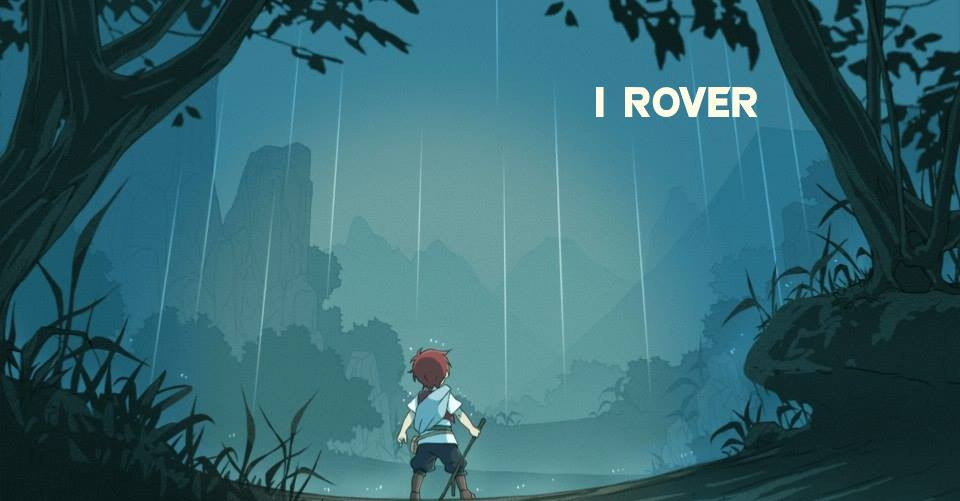
\includegraphics[width=350pt]{Illustration/proj_irover.jpg}
	\caption{iRover, l'histoire d'un héros qu'on appellait robot}
\end{figure}



\newpage


\renewcommand{\contentsname}{Sommaire} 
\tableofcontents

\newpage








\section{Rapport de Projet}


\vspace{2cm}



\subsection{Introduction}

\vspace{1 cm}


Le projet a pour objectif la création d'une application graphique où un petit personnage (robot) réaliserait une tache particulière.\\
Pour cela nous avons imaginé un scénario de mini jeu semblable au jeux en deux dimensions où notre robot prendrait la forme d'un héros sans peur et sans reproche.\\
L'autre aspect de ce projet est de pousser notre groupe à utiliser, comprendre et intégrer les autotools.
\vspace{1 cm}


\subsection{Membre du groupe et tâches de chacun}
\vspace{1 cm}

Le projet s'articule sur 5 grands pôles :

\vspace{1 cm}

\begin{tabbing}
\hspace{3.75 cm} \= \hspace{6 cm} \= \hspace{3.75 cm} \= \kill
\textbf{Pôle}\> \textbf{Description} \> \textbf {Responsable} \\
\\
Définition de la Carte \> La création de l'environnement \> Clément Bauchet\\											
Définition du robot \> Définitions de code de chaque \> Geoffrey Desbrosses\+ \\
élément de l'application. \- \\
IHM \> Interface utilisateur de l'application.\\
IA  \> Définitions des algorithmes \> Jean-Christophe Gambino Guerin \+ \\	
de déplacement et de découverte \-	\\
Documentation  \> Redaction de la documentation \> Joachim Clayton                           
\end{tabbing}





\newpage
\section{Définition de la Carte}


%partie de Clément

%mettre une petite introduction et parlez de vos parties


\newpage
\section{Définition du robot}

%partie Geoff
%mettre une petite introduction et parlez de vos parties

\subsection{code en c++(trouve un titre geoff xD)}
\subsection{gestion des évênements}

\section{IHM}


\newpage
\section{IA}

%partie JC
%mettre une petite introduction et parlez de vos parties

\subsection{path finding}
\subsection{découverte de la carte}


\newpage
\section{Problèmes rencontrer}


\section{Conclusion}



\end{document}

